\section{Theorie}
\label{sec:Theorie}

In dem Versuch soll ein Geiger-Müller-Zählrohr analysiert werden.
Dieses ist schematisch in der Abbildung \ref{fig:geiger} dargstellt worden.
Es besteht aus einem positiv geladenem Stab, welcher in der Mitte einer runden negativ geladenen Röhre sitzt. 
Die Röhre ist mit einem Edelgas-Alkohol Gemisch gefüllt.
Der Druck in der Röhre ist dabei allerdings stets niedriges als der Atmossphärendruck.
Das Rohr wird mit einer dünnen Mylar Schicht abgeschlossen, sodass das Gas nicht ausdringen kann.
Die Schicht aus Mylar wird benötigt, da diese durchlässig für radioaktive Strahlung also $\alpha$- $\beta$- oder $\gamma$-Teilchen ist.
\\\\
Trifft nun eins dieser radioaktiven Teilchen auf ein Gas Atmon so wird dieses ionisiert.
Da das Atom nun nicht mehr neutral geladen ist, folgt dies dem elektrischem Feld zwischen Anodenstab und Aussenwand.
Soabald es dort auftrifft entlädt sich das Atom wieder.
Dadurch ist es erneut neutral geladen.
Durch diesen Prozess entseht ein Spannungsunterschied zwischen Anodenstab und der Kathode, welche die Aussenwand bildet.
Dieser Unterschied ist allerdings zu gering und nicht messbar.
Nun kann es aber bei genügernd hoher Spannung dazu kommen, dass die Elektronen welche bei der Ionisierung des Atoms gelöst wurden, ein weiteres Atom ionisieren.
In diesem Fall nimmt die Anzahl des Ionisierungen exponetiell zu.
In diesem Zusammenhang wird von einer Townsend-Lawine gesprochen.
Hier ist die Spannungsdifferenz messbar und lässt sich durch ein Osziloskop visuel oder durch andere Vorrichtung akustsich bemerkbar machen.
Die Ladungsmenge welche durch ein Teilchen freigesetzt wird kann durch 
\begin{equation}
    Z = \frac{I}{Ne}
    \label{eq:z}
\end{equation}
berechnet werden.
$I$ ist dabei der Strom des Zählrohrs, $N$ die Anzahl der gemessenen Impulse über einen Zeitraum $t$ und $e$ die Elektronen Ladung.
Wenn das Zählrohr mit Betriebsspannung genutzt wird, kommt es zusätzlich zu den Townsend-Lawinen, noch dazu, dass UV-Photonen emittiert werden.
Da diese Ladungsneutral sind, können sie sich auch gegen die Feldrichtung des elektrischen Feldes bewegen und so Atome im gesamtem Rohr ionisieren.
\\\\
Durch die geringe Masse der Elektronen, bewegen sich diese schnell zum Anodendraht.
Da die Atome aber eine wesentlich höhere Masse als die Elektronen haben, halten sie sich wesentlich länger in der Gaskammer auf.
So entsteht ein positiv geladener Ring um den Anodendraht herum.
Durch diesen können kaum neue Atome ionisiert werden, was dazu führt, dass Teilchen die in dieser Zeit in das Rohr kommen nicht registriert werden.
Der Zeitraum in dem keine Registrierung möglich ist wird Totzeit $T$ des Zählrohrs genannt.
Die Totzeit eines Geiger-Müller-Zählrohrs kann mithilfe der Zwei-Quellen-Methode bestimmt werden.
Dazu wird die Differenz der Impulse genutzt, die ein Zählrohr zwischen der Messung von zwei einzelnen Quellen und beiden Quellen zusammen aufweist.
Die Totzeit kann so durch
\begin{equation}
    T \approx \frac{N_1+N_2-N_{1+2}}{2N_1 N_2}
    \label{eq:totzeit}
\end{equation} 
approximiert werden.
$N_1$ und $N_2$ sind dabei jeweils die gemessenen Impulse der einzelnen Quellen und $N_{1+2}$ ist die Anzahl der Impulse von beiden Quellen zusammen.
Der Messprozess und Ablauf ist ausführlich in Abschnitt \ref{subsec:tot} beschrieben worden.
\\\\
Wenn nun die registriert Teilchenzahl $N$ gegen die genutzte Spannnung $U$ aufgetragen wird entsteht die sogennante Charakteristik.
Eine schematische Darstellung einer Charakteristik ist in Abbildung \ref{fig:schemcharak} zu sehen.
Der mit 'Arbeitsbereich des Zählrohr' makierte Bereich entspricht dem Plateau, dessen Steigung im Abschnitt \ref{subsec:auscharak} berechnet wird.
Denn die Steigung des Plateau gibt an wie viele Nachentladungen im Zählrohr entstehen.
Diese sind im Allgemeinen unerwünscht, weswegen sich in den meisten Geiger-Müller-Zählrohren zusätzlich zu dem Edelgas, Alkohol befindet.
Dieser verhindert die Nachentladungen da diese mit den ionisiert Edelgas-Atomen zusammenstoßen.
Hierdurch werden die Alkohol Atome ionisiert, da ihre Ionisierungensenergie kleiner ist als die der Edelgas-Atome.
So wandern die Alkohol-Atome, anstatt der Edelgas-Atome, zur Kathode, wo sie neutraliesiert werden.
Vor dem Plateau ist auch die Spannung $U_\text{E}$ in der Grafik makiert worden, bei der der Auslösebereich des Geiger-Müller-Zählrohrs beginnt.
Hinter dem Plateau ist die Spannung am Zählrohr so groß, dass es zu einer Dauerentladung kommt, welche der Apparatur schadet.

\begin{figure}
    \centering
    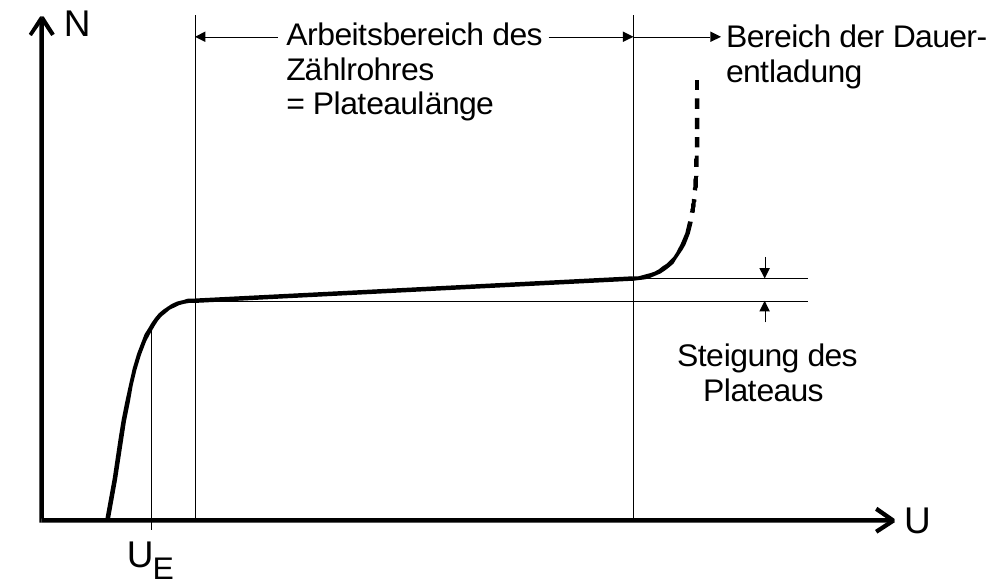
\includegraphics[width=0.6\textwidth]{content/data/charak.png}
    \caption{Die Charakteristik eines Geiger-Müller-Zählrohrs. Bild entnommen aus \cite{anleitung}.}
    \label{fig:schemcharak}
\end{figure}

\begin{figure}
    \centering
    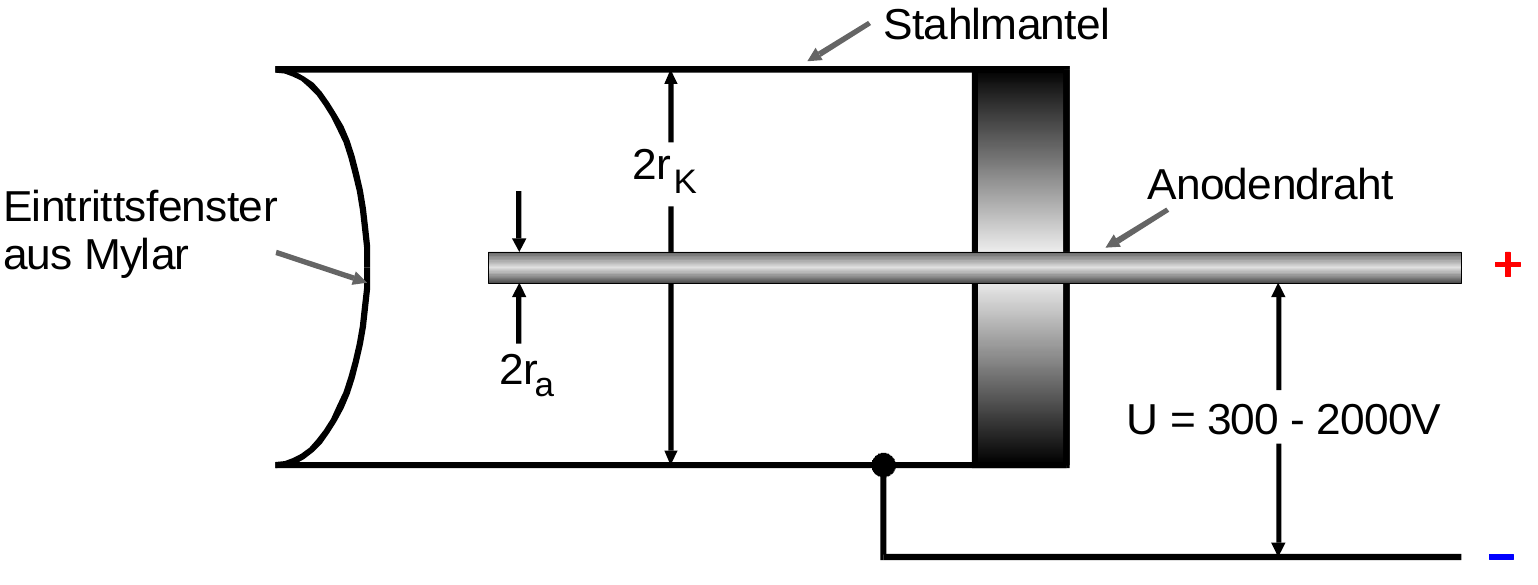
\includegraphics[width=0.6\textwidth]{content/data/rohre.png}
    \caption{Der schematisch Aufbau eines Geiger-Müller-Zählrohrs. Bild entnommen aus \cite{anleitung}.}
    \label{fig:geiger}
\end{figure}